\documentclass[]{article}

\usepackage{amsmath,amsthm,amssymb}
\DeclareMathOperator{\project}{project}
\DeclareMathOperator{\prox}{prox}
\DeclareMathOperator{\argmax}{argmax}
\DeclareMathOperator*{\minimize}{minimize}
\DeclareMathOperator*{\argmin}{arg\,min}

%\usepackage{program}
\usepackage{algorithm} 
\usepackage{algcompatible}
\usepackage{algpseudocode}

\usepackage[parfill]{parskip} % paragraphs are seperated with an enter space

\usepackage{graphicx}
\graphicspath{{./figs/}}

%opening
\title{A simple introduction to PANOC}
\author{Willem Melis}
\date{\today}

\begin{document}

\maketitle
\begin{abstract}
This is a simple introduction to solving an NMPC problem with the PANOC algorithm. First the proximal operator is introduced with the proximity gradient decent algorithm. Next the link is made between these algorithms and the PANOC algorithm.
\end{abstract}

\newpage
\tableofcontents 
\newpage

\section{Optimal control}

\section{MPC}
	\subsection{System}
		A physical system can be represented as $\dot{x}=F_c(x,u)$, where x is the current state and u is the current input. By using a discrete integrator the system can be written as $x^{k+1}=F_d(x^{k},u^{k})$. $F_d$ should be expressible as an series of elementary operations.
	\subsection{Problem definition}
		\subsubsection{Problem form}
			The goal is to define the problem as \eqref{eq:PANOC MPC form}, and then solve it for u given $x_0$, the current state of the system. Sometimes $x_0$ will be assumed to be part of the function f and the form of \eqref{eq:PANOC form} will be used.
			\begin{equation}
				\underset{u}{\minimize} \  f(x_0,u) + g(u)
				\label{eq:PANOC MPC form}
			\end{equation}
			
			\begin{equation}
				\underset{u}{\minimize} \  f(u) + g(u)
				\label{eq:PANOC form}
			\end{equation}
		\subsubsection{Single shoot}
			If the horizon is N then the problem is solved for the inputs $u=[u_0,u_1,... u_{N-1}]$ where each $u_k$ is a vector of all the inputs of the system. This means that the vector u is of size (Horizon-1)*dimension\_input .
			
			Define the cost for each step in the horizon as \eqref{eq:single shot iteration cost}.
			\begin{equation}
				\begin{aligned}
				& l_k(x_0,u) = &&  x_k^T Q x_k  +  u_k^T R u_k \\
				& \text{subject to}			&& x_0 = \bar{x} \\
				& 							&&  x_{n+1} = F_d(x_n,u_n), n=0...N-1
				\end{aligned}
				\label{eq:single shot iteration cost}
			\end{equation}
			
			Define the terminal cost as \eqref{eq:single shot terminal cost}.
			\begin{equation}
			\begin{aligned}
			& l_N(x_0,u) = && x_N^TSx_N \\
			& \text{subject to}			&& x_0 = \bar{x} \\
			& 							&&  x_{n+1} = F_d(x_n,u_n), n=0...N-1
			\end{aligned}
			\label{eq:single shot terminal cost}
			\end{equation}
			
			$f(x_0,u)$ can then be defined as in \eqref{eq:single shot definition} the sum of the cost of all iterations plus the terminal cost.
			\begin{equation}
				f(x_0,u) = \sum_{k=1}^{N-1} l_k(x_0,u) + l_N
				\label{eq:single shot definition}
			\end{equation}
			
			As a side note, an other term can be added to \eqref{eq:single shot definition} to represent the obstacle avoidance.
		\subsection{Multiple shoot}
			In multiple shoot mode the optimization algorithm needs more than just an initial state. It requires a guess of all of the intermediate states that where derived using the initial state in  single shot mode. The initial guesses will be referred to as $x_i$ and the states derived from this initial gas and its corresponding input will be referred to as $\bar{x_i}$. As before the goal of the optimization algorithm is to find the optimal inputs $u_i$, so that $\bar{x_i}$ is optimal.
			
			\begin{equation}
				\bar{x_i} = F(x_i,u_i)
				\label{eq:}
			\end{equation}
			
			In addition to getting the states to a specific reference state, the algorithm also needs continuity conditions. These continuity conditions are displayed in \eqref{eq:continuety condition multiple shot} and were not necessary in single shot as every solution already complies with it automatically. If the initial state guesses are relatively close to the solution, a significant speed increase can be accomplished. As we are able to incorporate more information into the algorithm.
			
			\begin{equation}
				\bar{x_i} - x_{i+1} = 0
				\label{eq:continuety condition multiple shot}
			\end{equation}
			
			The final cost definition looks like \eqref{eq:multiple shot cost} and has an extra equality condition compared to the single shoot. This equality condition will be added as a soft constraints to the cost function. This is displayed in \eqref{eq:multiple shot cost with soft constraint}
			
			\begin{equation}
				\begin{aligned}
				L =  & \sum_{i=1}^{N} l(\bar{x_i},u_i) \\
				& \text{subject to}			&& \bar{x_i} = F(x_i,u_i) \\
				& 							&& \bar{x_i} - x_{i+1} = 0
				\end{aligned}
				\label{eq:multiple shot cost}
			\end{equation}
			
			\begin{equation}
			\begin{aligned}
			L =  & \sum_{i=1}^{N} l(\bar{x_i},u) + ||\bar{x_i} - x_{i+1}||\\
			& \text{subject to}			&& \bar{x_i} = F(x_i,u_i) \\
			\end{aligned}
			\label{eq:multiple shot cost with soft constraint}
			\end{equation}
			
		\subsection{Obstacle avoidance}
			The obstacle avoidance is based on the soft constraint described in \cite{AjaySathya2017}.
			\subsubsection{As set}
				An obstacle can be defined as an open set, as illustrated by \eqref{eq:obstacle as open set}. It is defined by the intersection of a number of nonlinear inequalities.
				\begin{equation}
					O = {z \in \Re^d : h^i(z)>0,\ i \in N}
					\label{eq:obstacle as open set}
				\end{equation}
				
			\subsubsection{As constraint}
				\begin{equation}
					[z]_+ =  \max\{0,z\}
				\end{equation}
				
				The statement $h(x)<0$ is equivalent to saying $[h(x)]_+=0$,so ref{eq:obstacle as open set} is equivalent to saying that \eqref{eq:obstacle as equality} needs to be zero.
				
				\begin{equation}
					\Phi_0(z) =  \frac{1}{2} \prod_{i=1}^m \Big( [h^i(z)]_+ \Big)^2
					\label{eq:obstacle as equality}
				\end{equation}
				
				The gradient of \eqref{eq:obstacle as equality} is define as \eqref{eq:obstacle as equality}
				
				\begin{equation}
					\nabla \Phi =
					\begin{cases}
						\sum_{i=1}^{m} h^i(z)\prod_{j \ne i} \Big( [h^i(z)]_+ \Big)^2 \nabla h^i(z)
						& x \in O \\
						0 & else
					\end{cases}
					\label{eq:derivative obstacle as equality}
				\end{equation}
			
			\subsubsection{Polyhedral obstacle}
				A simple obstacle can be defined as \eqref{eq:polyhedral constraint} a polyhedral.
				\begin{equation}
					\prod \Big([b_i - a_i^t z]_+ \Big)^2 = 0
					\label{eq:polyhedral constraint}
				\end{equation}
			
			\subsubsection{Obstacle as soft constraint}
				The obstacle avoidance is added as a soft constraint to the cost function. As demonstrated in \eqref{eq:derivative obstacle as equality}, the gradient is defined and so this does not break the condition that the cost functions needs a gradient to be solved with the PANOC algorithm.
			
		\subsection{Constraints}
			An other important aspect of a MPC problem are the constraints. In practice inputs have to comply with the physical properties of the devices. Absurdly high or low input values might in theory lead to a fast solution, but are not feasible in practice.
			
			An major advantage of the PANOC algorithm is that it can take non linear or non convex constraints. As longs as the proximal operation is analytically defined on the constraint. 
			
			A simple example is the indicator box function, which allows to set a maximum and minimum value on the inputs. (The indicator box function is defined in the appendix) This means that every feasible solution lies within the bounds of the user defined box.
\chapter{Proximal gradient method}
	\subsection{Proximal mapping}
		The proximal operator is defined as $\prox_g(x)= \underset{u}{\argmin}(g(u) + \frac{1}{2 \gamma}||u-x||^2_2)$. 
		
		\begin{itemize}
			\item if $h(x)=0$ then $\prox_h(x)=x$ 
			\item if $h(x)=I_c(x)$ where $I_c$ is define in \eqref{eq:indicator function}, the proximity operator on an indicator function is the orthogonal projection on the set.
		\end{itemize}
		
		The indicator function: is defined in equation ~\eqref{eq:indicator function}.
		\begin{equation}
			I_c = 
			\begin{cases}
			0 & x \in C  \\
			\infty & x \notin C
			\end{cases}
			\label{eq:indicator function}
		\end{equation}
		
		The proximal mapping can be seen as a generalization of a projection. The Appendix contains an other important example, the indicator box function.
	
	\subsection{Gradient projected method}
		
		\begin{equation}
			\begin{aligned}
			& \underset{x}{\text{argmin}}
			& & f_0(x) \\
			& \text{subject to}
			& & g(x)=0
			\end{aligned}
			\label{eq:prox grad opti problem}
		\end{equation}
		
		The classical gradient decent method cannot be used to solve the problem of \eqref{eq:prox grad opti problem}. As this problem has a condition that must be met by the algorithms solution. If in each iteration the solution is projected on the space spanned by $g(x)=0$ the iteration \eqref{eq:grad descent} becomes \eqref{eq:projected grad descent}. This algorithm is called the gradient projection method.
		
		\begin{equation}
			x^k = x^{k-1} - \gamma \nabla f(x^{k-1})
			\label{eq:grad descent}
		\end{equation}
		
		\begin{equation}
			x^k = \project_{g(x)=0}[ x^{k-1} - \gamma \nabla f(x^{k-1})]
			\label{eq:projected grad descent}
		\end{equation}
		
		If $g(x)$ is the indicator function of the set onto which is projected. Then  \eqref{eq:projected grad descent} can be written as \eqref{eq:proximal grad descent}, known as the proximal gradient method.
		
		\begin{equation}
				x^k = \prox_{\gamma g}[ x^{k-1} - \gamma \nabla f(x^{k-1})]
			\label{eq:proximal grad descent}
		\end{equation}
	
	\subsection{The proximal gradient method}
		\eqref{eq:prox grad problem} Can be solved with the proximal gradient method, sometimes called forward backward splitting - FBS . Where the proximal mapping of $g(x)$ is analytically defined. 
			\begin{equation}
			\underset{x}{\argmin} = f(x) + g(x)
			\label{eq:prox grad problem}
			\end{equation}
		
		Inspired by the projected gradient method, the proximal gradient method is defined as \eqref{eq:prox grad method}. The $\gamma$ variable is the step size, in order to have a convergence of O(1/k) $\gamma \in(0,1/L)$. If $\gamma \in (1/L,2/L)$ the algorithm will still converge but then its no longer a majorization-minimization method. (more on this see \cite{NealParikh})
		
		\begin{equation}
			x^k = \prox_{\gamma g}\big( x^{(k-1)}- \gamma \nabla f(x^{(k-1)})\big)
			\label{eq:prox grad method}
		\end{equation}	
	
	\subsection{Proximal minimization algorithm}
		 \cite{QianYang} Contains a short proof that illustrates the proximal mapping as a fixed point minimization algorithm. A property of the conjugated function is used to derive the gradient, see appendix for the theorem.
		 \begin{proof}
		 	the iteration $x^{k+1}=\prox_g(x^k)$ will minimize the smoothed version of function f(x) 
		 	\begin{align*}
		 	f_{\mu}
		 	&= \underset{y}{\inf}\Big\{ |y| +\frac{1}{2 \mu}(x-y)^2 \Big\} \\
		 	&=   \frac{1}{2 \mu}||x||^2 + \frac{1}{2\mu} 
		 	\underset{y}{\inf}\Big\{
		 	2 \mu f(y) - 2x^T y + ||y||^2
		 	\Big\} \\
		 	&=  \frac{1}{2 \mu}||x||^2 + \frac{1}{\mu} 
		 	\underset{y}{\sup}\Big\{
		 	x^T y  - \mu f(y) - \frac{1}{2} ||y||^2 \Big \} \\
		 	&= \frac{1}{2\mu }||x||^2 \frac{1}{\mu } \Big( \mu f + \frac{1}{2}||\cdot||^2 \Big)^* (x) \\
		 	\nabla  f_{\mu} 
		 	&= \frac{x}{\mu} - \frac{1}{\mu} \underset{y}{\argmax} 
		 	\Big \{ x^Ty - \mu f(y) - \frac{1}{2}||y||^2 \Big \}\\
		 	& = \frac{1}{\mu}(x - \prox_{\mu f}(x)) \\
		 	\prox_{\mu f}(x)
		 	& = x- \mu \nabla f_{\mu}(x)
		 	\end{align*}
		 	\label{prf:proximal minimiztion alg proof}
		 \end{proof}

		 This means thats the iteration $x^{k+1}=\prox_g(x^k)$ will minimize the smoothed version of function g(x). 

\section{Proximal gradient method with line search}
	\subsection{Starting value gamma }
		\subsubsection{Estimating Lipschitz value}
			The Lipschitz of $\nabla f(x)$ value is a non negative number that complies with \eqref{eq:definition lipschitz value}.
			\begin{equation}
			L = \underset{x \neq y}{\sup} \frac{|\nabla f(y)-\nabla f(x)|}{|y-x|}
			\label{eq:definition lipschitz value}
			\end{equation}
			
			In practice it is not always possible to find the actual Lipschitz value. So the Lipschitz value is estimated ($L'$) locally at the starting location $x_0$ of the algorithm using \eqref{eq:estimated lipschitz value in starting position}. With $\delta=max[\delta_l,10^{-6} \cdot x_0]$ where $\delta_l$ is a small number chosen by the controller designer.
			% in code the safety value is DELTA_LIPSCHITZ_SAFETY_VALUE and set to 10^-6
			
			\begin{equation}
			L' = \frac{|\nabla f(x_0+\delta)-\nabla f(x_0)|}{|\delta|}
			\label{eq:estimated lipschitz value in starting position}
			\end{equation}
			
			The Lipschitz value is not explicitly saved but is used to estimate the line-search parameter $\gamma$. The backtracking of the proximal gradient descent then further improves this estimate. As the algorithm progresses and $\gamma$ improves, so does the estimation of the Lipschitz value indirectly.
		
		\subsubsection{Estimating gamma}	
			From \cite{LorenzoStella2017} it is known that $\gamma<\frac{1}{L}$ in order to guarantee convergence to a local minimum. As gamma needs to be smaller than $\frac{1}{L}$ a safety value is introduced. This idea was copied over from the kul-forbes/ForBES library by Lorenzo Stella and Panos Patrinos, which uses a $\beta$ of 0.05. And leads to \eqref{eq:starting value gamma}.
			\begin{equation}
			\gamma = \frac{1-\beta}{L}
			\label{eq:starting value gamma}
			\end{equation}		
	
	\subsection{Backtracking gamma}
		\subsubsection{Backtracking algorithm}
			Line-search is based on "Armijo's sufficient decrease condition" written down as \eqref{eq:Armijo's sufficient decrease condition}. The safety parameter $\theta$ multiplied with the step size $t_k$ is $\gamma=\theta \cdot t_k$. 
			
			\begin{equation}
			f(x_k + t_kp_k) \leq f(x_k) + \theta t_k \nabla f(x_k)^Tp_k
			\label{eq:Armijo's sufficient decrease condition}
			\end{equation}
			
			Line-search more specific backtracking will reduce the value of $\gamma$ until the condition of \eqref{eq:Armijo's sufficient decrease condition} fails.
			
		\subsubsection{Backtracking in proximal gradient descent used in FBS}
			The  "Armijo's sufficient decrease condition" is adjusted to \eqref{eq:Armijo's sufficient decrease condition prox grad PANOC} Which is an quadratic bound, $-p_k=x-\bar{x}$ and an additional term $\frac{1-\beta}{2 \gamma}||x-\bar{x}||^2$ is added.
			
			\begin{equation}
			f({\bar{x}}) \leq f(x) - \nabla f(x)^T[x-\bar{x}] + \frac{1}{2 \gamma}||x-\bar{x}||^2
			\label{eq:Armijo's sufficient decrease condition prox grad PANOC}
			\end{equation}
			
			This all leads to algorithm~\ref{alg:backtracking on gamma} the proximal gradient method. \eqref{eq:Armijo's sufficient decrease condition prox grad PANOC} can be seen as a quadratic model, as the Lipschitz value of the gradient is equal to $L=\frac{1}{\gamma}$.
			
			\begin{algorithm}
				\caption{backtracking $\gamma$}
				\label{alg:backtracking on gamma}
				\begin{algorithmic}[1]
					\Procedure {lineasearch\_gamma}{x,$\gamma$}
					\State $\bar{x} = \prox_{\gamma g}\big( x- \gamma \nabla f(x)\big)$
					\While{$f({\bar{x}}) > f(x) - \nabla f(x)^T[x-\bar{x}] + \frac{1}{2 \gamma}||x-\bar{x}||^2$}
					\State $\gamma = \frac{\gamma}{2}$
					\State $\bar{x} = \prox_{\gamma g}\big( x- \gamma \nabla f(x)\big)$
					\EndWhile
					\State \Return $\gamma$
					\EndProcedure
				\end{algorithmic}
			\end{algorithm}
	\subsection{Final algorthm}
		The final algorithm~\ref{alg:proximal gradient PANOC with backtracking} delivers the upward direction. $x_{k+1}=x_k - direction$.
		\begin{algorithm}
			\caption{proximal gradient PANOC with backtracking}
			\label{alg:proximal gradient PANOC with backtracking}
			\begin{algorithmic}[1]
				\Procedure{get\_proximal\_gradient\_step}{x,$\gamma$}
				\State $\gamma$=LINESEARCH\_GAMMA($\gamma$)
				\State $\bar{x} = \prox_{\gamma g}\big( x- \gamma \nabla f(x)\big)$
				\State \Return direction=$[x-\bar{x}]$, $\gamma$
				\EndProcedure
			\end{algorithmic}
		\end{algorithm}
\section{Proximal gradient alternative view}
	\subsection{Majorization-minimization algorithm}
	A Majorization-minimization algorithm, is a type of algorithm that minimizes a surrogate function. The surrogate function is a approximation of the actual problem. And needs to have the conditions described in \eqref{eq:MM algorithm conditions}, where h(x,y) is a surrogate function and f(x) is the actual problem. The problem described in \eqref{eq:MM algorithm formula step} is iteratively solved until convergence.
	\begin{equation}
		\begin{cases}
			h(x,x) = f(x) \\
			h(x,y) \leq f(x)
		\end{cases}
		\label{eq:MM algorithm conditions}
	\end{equation}
	
	\begin{equation}
		x_{k+1} = \argmin_y h(x_k,y)
		\label{eq:MM algorithm formula step}
	\end{equation}

	\subsection{The proximal gradient as majorization-minimization algorithm}
	The proximal gradient algorithm can be seen as a majorization-minimization algorithm. Its surrogate function is described in \eqref{eq:surrogate function}, proof~\ref{prf:proximal gradient as MM} illustrates how minimizing the surrogates function is equal as taking a step of the proximal gradient algorithm.
	
	\begin{equation}
		h(x,y) = f(x) + \nabla f(x)^T(x-y) + \frac{1}{2 \cdot \gamma}||x-y||^2_2
		\label{eq:surrogate function}
	\end{equation}
	
	\begin{proof}
		$h(x,y) = f(x) + \nabla f(x)^T(x-y) + \frac{1}{2 \cdot \gamma}||x-y||^2_2$ is the MM surugate function of proximal gradient algorithm. The gradient is set too zero and solved for y.
		\begin{align*}
		h(x,y)
		& = f(x) + \nabla f(x)^T(x-y) + \frac{1}{2 \cdot \gamma}||x-y||^2_2 \\
		\frac{\partial h(x,y)}{\partial y}
		& = 0 + \nabla f(x) + \frac{1}{2 \cdot \gamma} + \frac{1}{2 \cdot \gamma}\frac{\partial ||x-y||^2_2}{\partial y}  \\	
		\frac{\partial ||x-y||^2_2}{\partial y}
		& = \frac{\partial(x-y)^T(x-y)}{\partial y} = \frac{\partial(-2x^Ty + y^Ty)}{\partial y} = -2x+y \\
		\frac{\partial h(x,y)}{\partial y}
		& = \nabla f(x) - \frac{x}{\gamma} + \frac{y}{2 \gamma} = 0 \\
		0
		& = \gamma \nabla f(x) - x + \frac{y}{2} \\
		y & = \gamma \nabla f(x) - x
		\end{align*}
		\label{prf:proximal gradient as MM}
	\end{proof}
\clearpage
\chapter{PANOC algorithm}
	This section is based on \cite{LorenzoStella2017} and \cite{AjaySathya2017}, the difference is that this text is focused implementation. And so the formula's often look slightly different. The Forward backward envelop part is based on \cite{Themelis}, which contains a slightly different algorithm that also uses the Forward backward envelop.
	\section{Introducing panoc}
		The PANOC algorithm is an accelerated version of the proximal gradient descent. The direction  $x-\bar{x}$ is a combination of the proximal gradient algorithm and second direction that makes use of curvature information. This second direction will hopefully accelerate the convergence of the algorithm.
		
		\begin{equation}
		x_{k+1} = x_k + (1-\tau_k)\cdot (x-\bar{x}) + \tau_k d_k
		\end{equation}
		
		The new term $\tau_kd_k$ should accelerate the convergence if $\tau_k\neq0$. The step $d_k$ is calculated using a quasi-newton algorithm. As a quasi-newton algorithm uses curvature information of the cost function, it uses information not available to a gradient descent based method. 
		
		Furthermore it has a super linear convergence rate when it gets close to the solution. Which is much faster then the sub-linear convergence of a gradient descent algorithm . On top of that, the quasi-newton method will not require extra function evaluations. Which are the major contributors to the costs of the algorithm.
		
	\section{Quasi newton method}
		\subsubsection{Problem definition}
			The iteration of equation~\ref{eq:prox grad method} can indirectly be used to solve the optimization problem.  By using the residue defined in equation~\ref{eq:residue prox grad method} a fixed point can be found. 
			
			\begin{equation}
			R_{\gamma}(x)= \frac{1}{\gamma}\left[ x - \prox_g( x - \nabla f(x)\gamma) \right]
			\label{eq:residue prox grad method}
			\end{equation}
			
			The solution of equation~\ref{eq:residue prox grad method} can be found trough the Newton iteration of equation~\ref{eq:newton iteration residual}. Where $H_k$ satisfies the inverse secant condition of equation~\ref{eq:newton iteration residual inverse secant}. As the implementation is aimed at embedded software a good option to solve this would be L-BFGS. More on this in the chapter on L-BFGS.
			
			\begin{equation}
			x^{k+1} = x^k -H_kR_{\gamma}(x^k)
			\label{eq:newton iteration residual}
			\end{equation}
			\begin{equation}
			x^{k+1} - x^k = H_{K+1} \Big( R_{\gamma}(x^{k+1})- R_{\gamma}(x^k) \Big)
			\label{eq:newton iteration residual inverse secant}
			\end{equation}
		
	\section{Forward backward envelop}	
		Newton iterations only converge quickly when they are close to the solution. In order to get better global behavior a proper global strategy is required. The optimization problem is changed from $\varphi(x) = f(x) + g(x)$ to equation~\ref{eq:FBE definition using Moreau envelope}. This problem is smoother while it still has the same optimal solution.(proof see \cite{LorenzoStella2017} and \cite{Themelis}) The same $\gamma$ as with the proximal gradient should be used, notice how the FBE contains the line-search condition use in the proximal gradient. (more on the FBE in \cite{Themelis})
		
		The Moreau envelope is de define as \ref{eq:Moreau envelope}, this smooths the function, and has a close relationship with the proximal operator as illustrated earlier. Using simple algebra equation~\ref{eq:FBE definition using Moreau envelope} can be transformed into equation~\ref{eq:FBE definition using quadratic approximation}.(proof in Appendix) The solution $y$ of the infimum defined in equation~\ref{eq:FBE definition using quadratic approximation} is $\bar{x}$. Considering the close relationship between the Moreau envelope and the proximal operator (see more in \cite{Themelis}) this is to be expected.
		
		An alternative way to look the FBE is illustrated in \cite{AjaySathya2017}, where the problem can be seen as minimizing a quadratic approximation  $f(x) +  \nabla f(x)^T(y-x) + g(y) + \frac{1}{2 \gamma} ||x-y||^2  $ towards y in point x.  Remember that $L = \frac{1}{\gamma}$, with L being the Lipschitz constant of the gradient.
		
		\begin{equation}
			g^{\gamma} = \underset{y}{\inf} \big \{f(y)+\frac{1}{2 \cdot \gamma}||x-y||^2 \big \}
			\label{eq:Moreau envelope}
		\end{equation}
		
		\begin{equation}
		\varphi_{\gamma} = f(x) - \frac{\gamma}{2}||\nabla f(x)||^2 + g^{\gamma} \big(x-\gamma \nabla f(x) \big)
		\label{eq:FBE definition using Moreau envelope}
		\end{equation}
		
		\begin{equation}
		\varphi_{\gamma} =   f(x) + \underset{y}{\inf} \Big\{ \nabla f(x)^T(y-x) + g(y) + \frac{1}{2 \gamma} ||x-y||^2  \Big\}
		\label{eq:FBE definition using quadratic approximation}
		\end{equation}
		
		\begin{proof}
			The solution to the infimum of equation~\ref{eq:FBE definition using quadratic approximation} is y=$\bar{x}= \prox_g(x-\gamma \nabla f(x))$
			\begin{align*}
			\prox_g(\bar{x}) 
			&=\prox_g(x- \gamma \nabla f(x)) \\
			&= \underset{y}{\argmin} \Big \{ g(y) 
			+ \frac{1}{2 \gamma}||(y-x) + \gamma \nabla f(x)||^2 \Big \} \\
			&= \underset{y}{\argmin} \Big \{ g(y) 
			+ \frac{1}{2 \gamma} \big[||y-x||^2 + 2 \gamma \nabla f(x)^T(y-x) + ||\nabla f(x)||^2\gamma^2 \big] \Big \} \\
			&= \underset{y}{\argmin} \Big \{ g(y) 
			+ \frac{1}{2 \gamma} \big[||y-x||^2 + 2 \gamma \nabla f(x)^T(y-x)  \big] \Big \}\\
			&= \underset{y}{\argmin} \Big \{   \nabla f(x)^T(y-x)  + g(y) 
			+ \frac{1}{2 \gamma} ||y-x||^2  \Big  \}
			\end{align*}
			\label{prf:prox is solution to FBE inf}
		\end{proof}
		
		Equation~\ref{eq:practical implementation of FBE} is the practical implementation of the FBE. The parameter gamma is the line-search parameter used in the proximal gradient descent. The first 3 terms are the same as with the line-search on $\gamma$, the last term $g(\bar{x})$ is new and makes sure the solution complies with the constraint.
		
%		\cite{AjaySathya2017} has an excellent example to illustrate this.(figure~\ref{fig:FBE illustration}).
%		
		\begin{equation}
			\begin{aligned}	
				& \varphi(\gamma,x)= 
				&& f(x) - \nabla f(x)^T(x-\bar{x}) + \frac{1}{2 \gamma}||x-\bar{x}||^2  + g(\bar{x})
				\\
				& with 
				&&\bar{x} = \prox_g( x - \gamma\nabla f(x)) 
			\end{aligned} 
			\label{eq:practical implementation of FBE}
		\end{equation}
		
%		\begin{figure}[H]
%			\centering
%			\label{fig:FBE illustration}
%			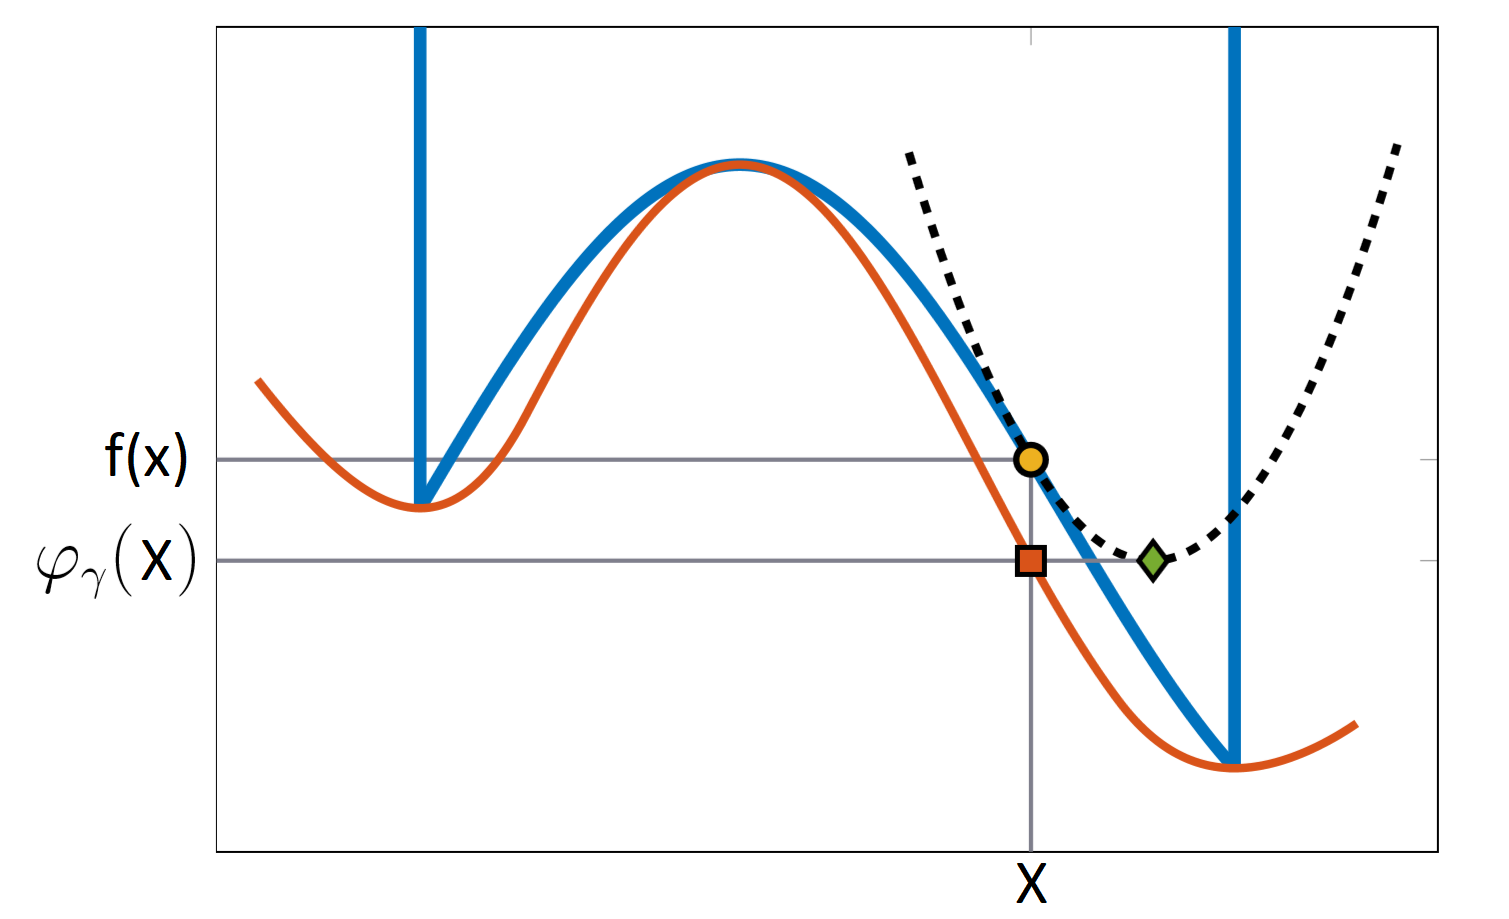
\includegraphics[width=0.6\textwidth]{FBE}
%			\caption{FBE example copied over from \cite{AjaySathya2017}, red is?? blue is ?? TODO expain this figure}
%		\end{figure}
	
	\section{Line-search with FBE}
	In \cite{LorenzoStella2017} the line-search condition is specified as equation ~\ref{eq:line-search with FBE}. The line-search parameter $\tau$ determines $x^{k+1}$ by choosing the convex combination of the step from the proximal gradient and the L-BGFS as defined in equation~\ref{eq:linea-search tau definition}.  \cite{LorenzoStella2017} specifies that $\sigma \in (0, \gamma \frac{1-\gamma\cdot L}{2})$. As stated before it is assumed that $L=\frac{1-\beta}{\gamma}$, some simple algebra will lead to the condition $\sigma \in (0,\frac{\beta \gamma}{2})$.
	
	 Equation~\ref{eq:practical line-search with FBE} is the practical implementation of equation~\ref{eq:line-search with FBE}. A new constant $\alpha \in (0,1)$ is introduced, an possible value for $\alpha$ would be 0.5 ($\alpha=0.5$ is the choice used by the Matlab implementation of PANOC in ForBes known as zerofpr2).
	
	\begin{equation}
		x^{k+1} = u_k - (1-\tau_k)\cdot (x-\bar{x}) + \tau \cdot dir_{LBFGS}
		\label{eq:linea-search tau definition}
	\end{equation}
	
	\begin{eqnarray}
		\label{eq:line-search with FBE}
		\varphi_{\gamma}(x^{k+1})\leq\varphi_{\gamma}(x^{k}) - \sigma ||\frac{x-\bar{x}}{\gamma}||^2 \\
		=
		\varphi_{\gamma}(x^{k}) - \frac{\sigma}{\gamma^2} ||x-\bar{x}||^2
	\end{eqnarray}
	
	\begin{equation}
		\varphi_{\gamma}(x^{k+1}) \leq 		\varphi_{\gamma}(x^{k}) - \alpha \frac{\beta }{\gamma \cdot 2} ||x-\bar{x}||^2
		\label{eq:practical line-search with FBE}
	\end{equation}
	
	
		
		\begin{algorithm}
			\caption{PANOC}
			\label{alg:PANOC}
			\begin{algorithmic}[1]
				\Procedure {PANOC\_GET\_NEW\_LOCATION}{$x^k$,$\gamma$}
				\State [$(x-\bar{x})$ , $\gamma$] = GET\_PROXIMAL\_GRADIENT\_STEP($\gamma$,$x^k$)
				\State $ dir_{LBFGS}$ = LBFGS($x^k$)
				\State $\tau =1$
				\State $x^{k+1} = x_k - (1-\tau_k)\cdot (x-\bar{x}) + \tau \cdot dir_{LBFGS}$
				\While{$\varphi_{\gamma}(x^{k+1}) > 		\varphi_{\gamma}(x^{k}) - \alpha \frac{\beta}{\gamma \cdot 2} ||(x-\bar{x})||^2$}
				\State $\tau = \tau / 2$
				\State $x^{k+1} = x_k - (1-\tau_k)\cdot (x-\bar{x}) + \tau \cdot dir_{LBFGS}$
				\EndWhile
				\EndProcedure
			\end{algorithmic}
		\end{algorithm}
	

\clearpage

\section{Implementation}
	\subsection{the dynamic C code}
	\subsection{The static C lib}
		The static c code is structured in an layered architecture. The PANOC algorithm is the first layer. PANOC calls the second layer containing the LBFGS and proximal gradient descent. And finally the lowest layer containing the Casadi functions, a buffer and the Lipschitz estimator.
		\begin{figure}[H]
			\centering
			\label{fig:software architecture}
			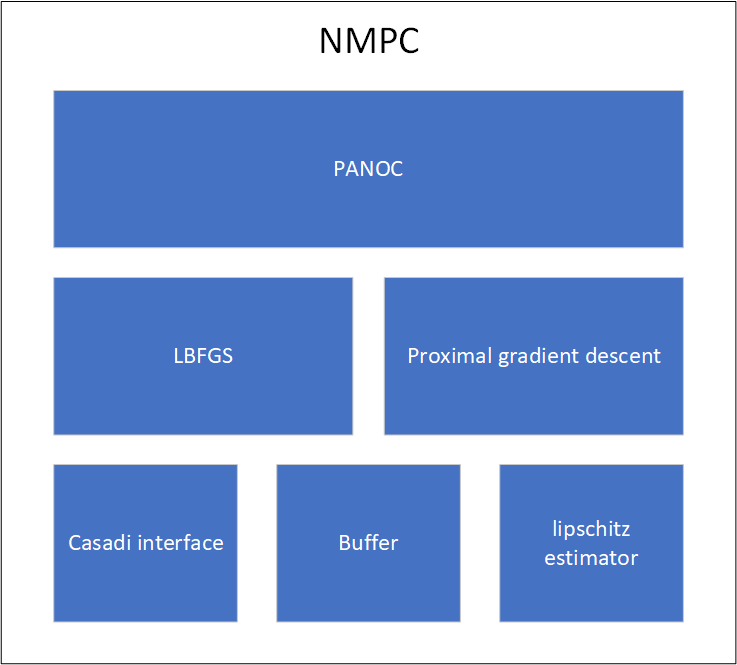
\includegraphics[width=0.8\textwidth]{visio_software_arch}
			\caption{software architecture}
		\end{figure}
	
\clearpage
\appendix 
\chapter{Abstract Dutch}
Moderne controle systemen maken vaak gebruik van "model predictive control" algoritmes. Wanneer lineaire modellen gebruikt worden, moet een stelsel van lineaire vergelijkingen worden opgelost. De algoritmes voor het oplossen van een stelsel van lineaire vergelijkingen zijn uitgebreid onderzocht en ge\"{i}mplementeerd. 

Wanneer een niet-lineaire model wordt gebruikt, moet een niet-lineaire stelsel opgelost worden. Dit stelsel kan worden opgelost met iteratieve algoritmes zoals "interior point" of SQP algoritmes. Deze algoritmes gebruiken veel geheugen, wat ze vaak ondergeschikt maken voor embedded toepassingen. Het "proximal gradient" algoritme gebruikt weinig geheugen maar heeft slechts sub lineaire convergentie. Dit is waar het PANOC algoritme interessant wordt, het kan namelijk een niet lineaire stelsel oplossen met veel minder geheugen dan een "interior point" algoritme. Maar heeft wel super lineaire convergentie. 

Het doel van deze masterproef is een raamwerk te implementeren die een niet-lineaire MPC controller genereert in C. De controller maakt gebruik van het PANOC algoritme voor het oplossen van het niet lineaire stelsel. De code is specifiek gericht aan embedded toestellen, waardoor PANOC een uitstekende keuze is. De gebruiker van de software wordt verondersteld alleen controletheorie te kennen, en hoeft niets over PANOC algoritme noch embedded software te kennen.

De implementatie is gerealiseerd in Matlab en Python, aangezien dit de twee dominerende talen zijn bij computer simulaties van controlesystemen. Er wordt geen gebruik gemaakt van externe bibliotheken om de C code te genereren. Het PANOC is een convexe combinatie van het "proximal gradient" algoritme en L-BFGS. Er wordt gebruik gemaakt van het pakket Casadi om de gradi\"{e}nt te berekenen. Het is mogelijk om vanuit Matlab of Pyhton simulaties uit te voeren op de gegenereerde C code. Zo kunnen de nodige controle parameters afgesteld worden vanuit Matlab of Python.

De gegenereerde C code is getest met de GNU C compiler, Clang LLVM compiler, Microsoft C compiler en de Intel C compiler onder de ANSI C89 standaard. Er worden geen externe C bibliotheken gebruikt zodat de code eenvoudig kan gecompileerd worden voor verschillende platformen. Het enige noodzakelijke is een C compiler.

Vervolgens wordt aangetoond dat PANOC bij eenvoudige systemen sneller is dan "interior point" methodes, maar bij complexe systemen verliest het zijn snelheids voordeel. PANOC verbruikt wel altijd minder geheugen.

Tot slot is er recentelijk onderzoek ge\"{i}mplementeerd. Het toevoegen van voorwaarden op het controlesysteem kan namelijk leiden tot een slecht geconditioneerd probleem. De "augmented Lagrangian" methode bied hiervoor een oplossing. Door het probleem in verschillende stappen op te lossen kan er soms een beter resultaat bereikt worden.

\chapter{Mathematical definitions}
	\section{Box function}
	\label{appendix:box function}
		1 dimension:
		\begin{equation}
			\boxfunction_{1D}(u) =
			\begin{cases}
				 1 & u \in [-U_b:U_b]\\
				 0 & \other
			\end{cases}
			\label{eq:box function 1 dimension}
		\end{equation}
		N dimensions:
		\begin{equation}
			\boxfunction(u) = \min\left[ \sum_{k=1}^ N \boxfunction_{1D}(u) \right]
			\label{eq:box function N dimensions}
		\end{equation}
	\section{Indicator Box function}
	\label{appendix:indicator box function}
		\begin{equation}
			I_{\boxfunction}(u)=
			\begin{cases}
				0 & u \in [-U_b:U_b]\\
				\inf & \other
			\end{cases}
		\end{equation}
		
		\begin{equation}
			\prox_{\gamma I_{\boxfunction}}(u)=
			\begin{cases}
				u & u \in [-U_b:U_b]\\
				-U_b & u \in [-\inf:-U_b)\\
				-U_b & u \in (U_b:\inf]\\
			\end{cases}
		\end{equation}
	\section{Conjugate of strongly convex function}
	\label{appendix:conjugate of strongly convex function}
		\begin{equation}
			f^*(x)= \underset{u \in dom(f)}{<y,x>-f(y)}
		\end{equation}
		
		If $\nabla f^*$ is Lipschitz and obeys \eqref{eq:appendix f lip}, then $f^*$ is well defined and differentiable. (assume dom(f) is convex and closed)
		\begin{equation}
			\nabla f^*(x) = y^* = \argmax <y,x> - f(y)
		\end{equation}
		
		\begin{equation}
			|| \nabla f^*(x) - \nabla f^*(y) ||_2 \leq \mu^{-1} ||x-y||_2
			\label{eq:appendix f lip}
		\end{equation}
		
\chapter{Proof FBE alternative equation}
\label{appendix:proof FBE alternate equation}
\begin{proof}
	$\varphi_{\gamma} =   f(x) + \underset{y}{\inf} \Big\{ \nabla f(x)^T(y-x) + g(y) + \frac{1}{2 \gamma} ||x-y||^2  \Big\} $
	\begin{align*}
	g^{\gamma} 	&=  \underset{y}{\inf} \big \{f(y)+\frac{1}{2 \cdot \gamma}||x-y||^2 \big \} \\
	\varphi_{\gamma} 
	&= f(x) - \frac{\gamma}{2}||\nabla f(x)||^2 + g^{\gamma} \big(x-\gamma \nabla f(x) \big) \\
	&= f(x) - \frac{\gamma}{2}||\nabla f(x)||^2 + g^{\gamma} \big(\bar{x} \big)\\
	g^{\gamma} (\bar{x})
	&=\underset{y}{\inf} \Big\{g(y)+\frac{1}{2 \gamma}||\bar{x}-y||^2 \Big\}	\\
	\bar{x}^T\bar{x}
	&=[x- \gamma \nabla f(x)]^T[x- \gamma \nabla f(x)] \\
	&= x^Tx -2x^T\nabla f(x) \gamma + \gamma^2 \nabla f(x)^T\nabla f(x)-2x^Ty \\
	&=-2x^Ty + 2\gamma \nabla f(x)^Ty \\
	\frac{1}{2 \gamma}||\bar{x}-y||^2
	&=\frac{1}{2 \gamma} \Big [ (\bar{x}-y)^T(\bar{x}-y) \Big]\\
	&=\frac{1}{2 \gamma} \Big [ x^Tx - 2 x^Ty + y^Ty \Big]\\
	& = \frac{1}{2 \gamma}[-2x^T\nabla f(x) \gamma  + 2\gamma \nabla f(x)^Ty + \gamma^2 \nabla f(x)^T\nabla f(x) +x^Tx -2x^Ty +y^Ty]\\
	&= \frac{1}{2 \gamma}[ 2\gamma \nabla f(x)^T(y-x) + \gamma^2||\nabla f(x)||^2 + ||x-y||^2] \\
	&=  \nabla f(x)^T(y-x) +\frac{\gamma}{2}||\nabla f(x)||^2 + \frac{1}{2 \gamma} ||x-y||^2 \\
	g^{\gamma} (\bar{x})
	&=\underset{y}{\inf} \Big\{g(y)+ \nabla f(x)^T(y-x) +\frac{\gamma}{2}||\nabla f(x)||^2 + \frac{1}{2 \gamma} ||x-y||^2  \Big\} \\
	&= \frac{\gamma}{2}||\nabla f(x)||^2 + \underset{y}{\inf} \Big\{g(y)+ \nabla f(x)^T(y-x) + \frac{1}{2 \gamma} ||x-y||^2  \Big\} \\
	\varphi_{\gamma} 
	&= f(x) - \frac{\gamma}{2}||\nabla f(x)||^2 + g^{\gamma} \big(\bar{x} \big)\\
	&= f(x) - \frac{\gamma}{2}||\nabla f(x)||^2 +  \frac{\gamma}{2}||\nabla f(x)||^2 + \underset{y}{\inf} \Big\{g(y)+ \nabla f(x)^T(y-x) + \frac{1}{2 \gamma} ||x-y||^2  \Big\}\\
	&=   f(x) + \underset{y}{\inf} \Big\{ \nabla f(x)^T(y-x) + g(y) + \frac{1}{2 \gamma} ||x-y||^2  \Big\} 
	\end{align*}
	\label{prf:FBE alterative expression}
\end{proof}

\chapter{Benchmarks with trailer model}
\label{appendix:paths trailer simulations}

\begin{figure}[H]
	\centering
	\begin{subfigure}[b]{0.40\textwidth}
		\centering
		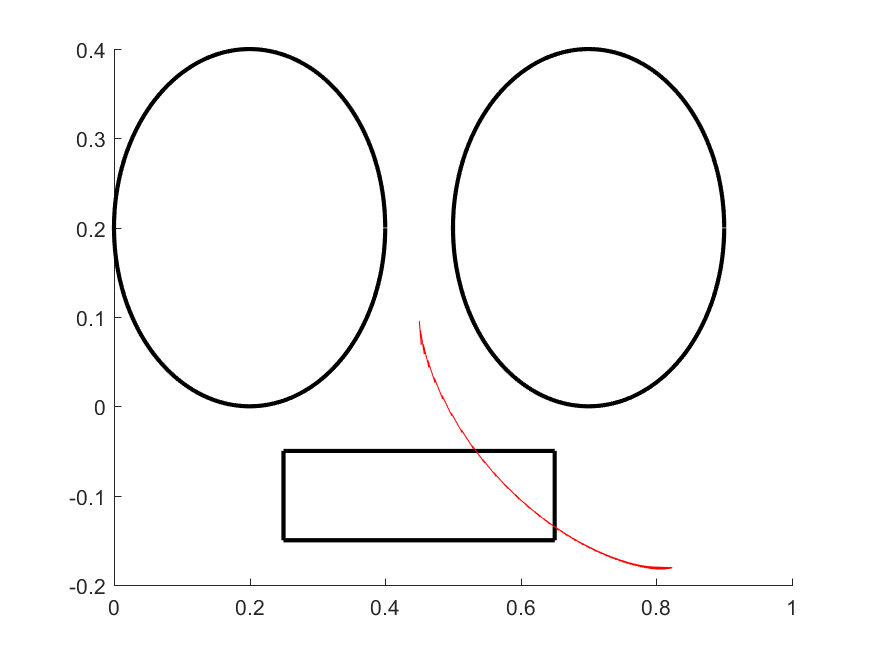
\includegraphics[width=1.2\textwidth]{demos/demo1}
		\caption{demo 1}
		\label{fig:demo 1}
	\end{subfigure}
	\hfill
	\begin{subfigure}[b]{0.40\textwidth}
		\centering
		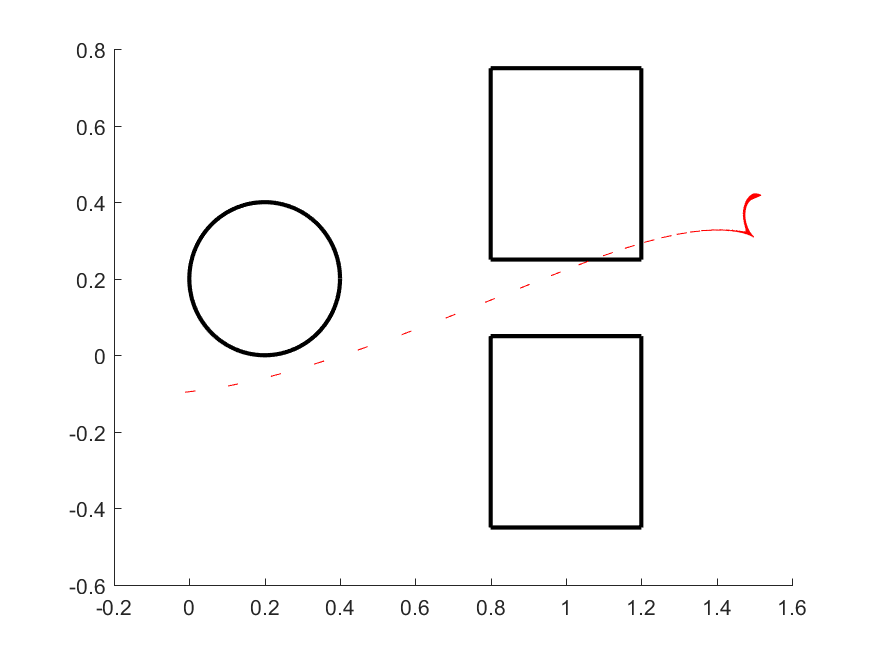
\includegraphics[width=1.2\textwidth]{demos/demo2}
		\caption{demo 2}
		\label{fig:demo 2}
	\end{subfigure}
	\begin{subfigure}[b]{0.40\textwidth}
		\centering
		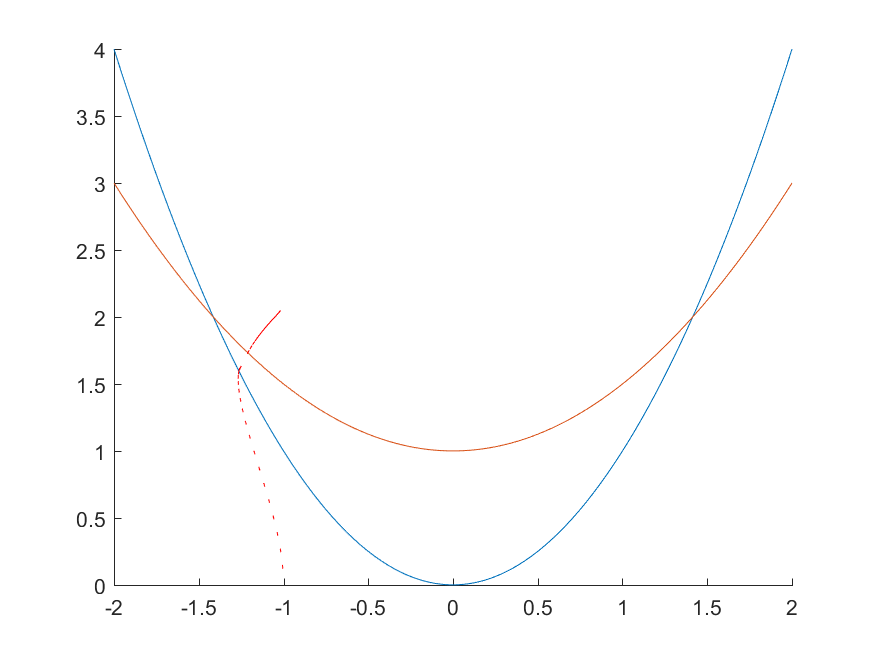
\includegraphics[width=1.2\textwidth]{demos/demo3}
		\caption{demo 3}
		\label{fig:demo 3}
	\end{subfigure}
	\hfill
	\begin{subfigure}[b]{0.40\textwidth}
		\centering
		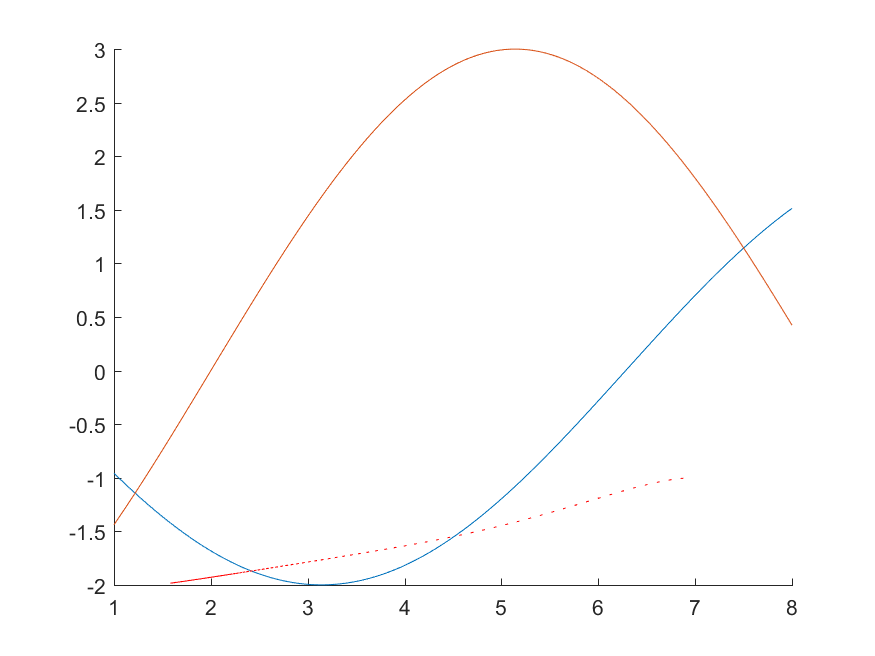
\includegraphics[width=1.2\textwidth]{demos/demo4}
		\caption{demo 4}
		\label{fig:demo 4}
	\end{subfigure}
	\caption{Path of demo's}
	\label{fig:demos}
\end{figure}
\begin{figure}[H]
	\centering
	\begin{subfigure}[b]{0.45\textwidth}
		\centering
		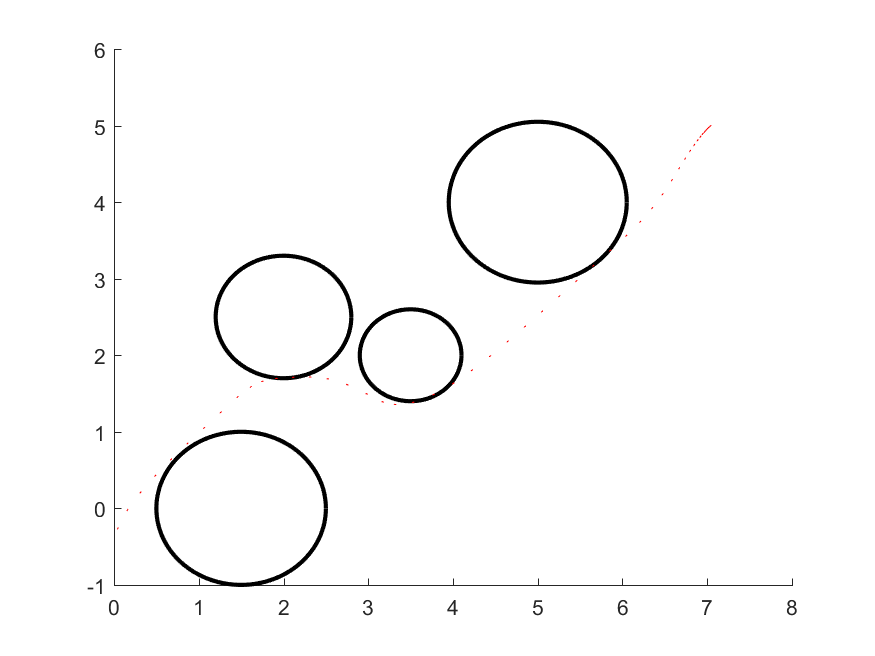
\includegraphics[width=1.2\textwidth]{demos/demo5}
		\caption{demo 5}
		\label{fig:demo 5}
	\end{subfigure}
\end{figure}

\section{Simulations without state noise}
\label{appendix:benchmarks trailer without noise}

\begin{table}[H]
	\centering
	\begin{tabular}{|l|c|c|c|c|}
		\hline
		&\textbf{demo5}&\textbf{demo2}&\textbf{demo3}\\\hline
		\textbf{nmpc-codegen (PANOC)}&9.00e-01&1.00e-01&4.10e-01\\\hline
		\textbf{ForBeS zerofrp2 (PANOC)}&2.99e+01&4.20e+00&5.56e+00\\\hline
		\textbf{PANOC draft}&5.73e+00&1.29e+00&2.00e+00\\\hline
		\textbf{fmincon:interior-point}&8.62e+01&2.31e+01&2.03e+01\\\hline
		\textbf{fmincon:sqp}&2.18e+01&1.15e+01&9.29e+00\\\hline
		\textbf{fmincon:active-set}&8.37e+01&2.36e+01&2.08e+01\\\hline
		\textbf{OPTI:ipopt}&3.79e+01&7.08e+00&8.21e+00\\\hline
	\end{tabular}
	\caption{mean time till convergence in milliseconds}
	\label{tbl:mean time till convergence}
\end{table}

\begin{table}[H]
	\centering
	\begin{tabular}{|l|c|c|c|c|}
		\hline
		&\textbf{demo5}&\textbf{demo2}&\textbf{demo3}\\\hline
		\textbf{nmpc-codegen (PANOC)}&100&100&100\\\hline
		\textbf{ForBeS zerofrp2 (PANOC)}&3323&4202&1357\\\hline
		\textbf{PANOC draft}&637&1289&489\\\hline
		\textbf{fmincon:interior-point}&9579&23107&4943\\\hline
		\textbf{fmincon:sqp}&2422&11469&2265\\\hline
		\textbf{fmincon:active-set}&9303&23578&5084\\\hline
		\textbf{OPTI:ipopt}&4213&7083&2003\\\hline
	\end{tabular}
	\caption{mean relative time till convergence in milliseconds}
	\label{tbl:mean relative time till convergence}
\end{table}

\begin{table}[H]
	\centering
	\begin{tabular}{|l|c|c|c|c|}
		\hline
		&\textbf{demo5}&\textbf{demo2}&\textbf{demo3}\\\hline
		\textbf{nmpc-codegen (PANOC)}&2.20e+01&8.00e+00&4.00e+01\\\hline
		\textbf{ForBeS zerofrp2 (PANOC)}&7.95e+02&1.25e+02&3.06e+02\\\hline
		\textbf{PANOC draft}&1.12e+02&3.66e+01&1.30e+02\\\hline
		\textbf{fmincon:interior-point}&1.55e+03&2.29e+02&2.95e+02\\\hline
		\textbf{fmincon:sqp}&1.01e+02&8.83e+01&1.10e+02\\\hline
		\textbf{fmincon:active-set}&7.83e+02&2.70e+02&2.45e+02\\\hline
		\textbf{OPTI:ipopt}&2.73e+02&4.65e+01&7.65e+01\\\hline
	\end{tabular}
	\caption{max time till convergence in milliseconds}
	\label{tbl:max time till convergence}
\end{table}

\begin{table}[H]
	\centering
	\begin{tabular}{|l|	c|c|c|c|}
		\hline
		&\textbf{demo5}&\textbf{demo2}&\textbf{demo3}\\\hline
		\textbf{nmpc-codegen (PANOC)}&0.00e+00&0.00e+00&0.00e+00\\\hline
		\textbf{ForBeS zerofrp2 (PANOC)}&2.11e+00&2.03e+00&2.01e+00\\\hline
		\textbf{PANOC draft}&5.16e-01&5.26e-01&5.16e-01\\\hline
		\textbf{fmincon:interior-point}&8.95e+00&8.35e+00&7.57e+00\\\hline
		\textbf{fmincon:sqp}&6.37e+00&6.58e+00&6.02e+00\\\hline
		\textbf{fmincon:active-set}&1.82e+01&1.63e+01&1.57e+01\\\hline
		\textbf{OPTI:ipopt}&5.03e+00&4.45e+00&4.37e+00\\\hline
	\end{tabular}
	\caption{min time till convergence in milliseconds}
	\label{tbl:min time till convergence}
\end{table}


\section{Simulations with state noise}
\label{appendix:benchmarks trailer with noise}

\begin{table}[H]
	\centering
	\begin{tabular}{|l|c|c|c|c|}
		\hline
		&\textbf{demo5}&\textbf{demo2}&\textbf{demo3}\\\hline
		\textbf{nmpc-codegen (PANOC)}&5.82e+00&4.20e-01&2.20e-01\\\hline
		\textbf{ForBeS zerofrp2 (PANOC)}&8.69e+01&1.19e+01&9.64e+00\\\hline
		\textbf{PANOC draft}&2.77e+01&4.54e+00&3.24e+00\\\hline
		\textbf{fmincon:interior-point}&3.17e+02&1.01e+02&8.15e+01\\\hline
		\textbf{fmincon:sqp}&9.07e+01&4.77e+01&3.93e+01\\\hline
		\textbf{fmincon:active-set}&2.29e+02&7.50e+01&6.46e+01\\\hline
		\textbf{OPTI:ipopt}&9.52e+01&1.41e+01&1.09e+01\\\hline
	\end{tabular}
	\caption{mean time till convergence in milliseconds}
	\label{tbl:mean time till convergence with noise}
\end{table}

\begin{table}[H]
	\centering
	\begin{tabular}{|l|c|c|c|c|}
		\hline
		&\textbf{demo5}&\textbf{demo2}&\textbf{demo3}\\\hline
		\textbf{nmpc-codegen (PANOC)}&100&100&100\\\hline
		\textbf{ForBeS zerofrp2 (PANOC)}&1494&2839&4383\\\hline
		\textbf{PANOC draft}&476&1080&1472\\\hline
		\textbf{fmincon:interior-point}&5453&24054&37058\\\hline
		\textbf{fmincon:sqp}&1560&11360&17870\\\hline
		\textbf{fmincon:active-set}&3937&17860&29378\\\hline
		\textbf{OPTI:ipopt}&1637&3362&4952\\\hline
	\end{tabular}
	\caption{mean relative time till convergence in milliseconds}
	\label{tbl:mean relative time till convergence with noise}
\end{table}

\begin{table}[H]
	\centering
	\begin{tabular}{|l|c|c|c|c|}
		\hline
		&\textbf{demo5}&\textbf{demo2}&\textbf{demo3}\\\hline
		\textbf{nmpc-codegen (PANOC)}&1.06e+02&1.30e+01&1.80e+01\\\hline
		\textbf{ForBeS zerofrp2 (PANOC)}&9.82e+02&2.23e+02&3.87e+01\\\hline
		\textbf{PANOC draft}&2.38e+02&7.07e+01&1.83e+01\\\hline
		\textbf{fmincon:interior-point}&2.45e+03&4.68e+02&3.40e+02\\\hline
		\textbf{fmincon:sqp}&4.22e+02&3.25e+02&4.18e+02\\\hline
		\textbf{fmincon:active-set}&1.13e+03&4.86e+02&5.69e+02\\\hline
		\textbf{OPTI:ipopt}&4.78e+02&9.21e+01&3.67e+01\\\hline
	\end{tabular}
	\caption{max time till convergence in milliseconds}
	\label{tbl:max time till convergence with noise}
\end{table}

\begin{table}[H]
	\centering
	\begin{tabular}{|l|	c|c|c|c|}
		\hline
		&\textbf{demo5}&\textbf{demo2}&\textbf{demo3}\\\hline
		\textbf{nmpc-codegen (PANOC)}&0.00e+00&0.00e+00&0.00e+00\\\hline
		\textbf{ForBeS zerofrp2 (PANOC)}&4.62e+00&3.55e+00&3.18e+00\\\hline
		\textbf{PANOC draft}&1.80e+00&1.26e+00&1.22e+00\\\hline
		\textbf{fmincon:interior-point}&4.85e+01&1.33e+01&1.05e+01\\\hline
		\textbf{fmincon:sqp}&1.44e+01&8.63e+00&9.95e+00\\\hline
		\textbf{fmincon:active-set}&3.48e+01&2.04e+01&1.72e+01\\\hline
		\textbf{OPTI:ipopt}&1.68e+01&4.67e+00&5.38e+00\\\hline
	\end{tabular}
	\caption{min time till convergence in milliseconds}
	\label{tbl:min time till convergence with noise}
\end{table}

\chapter{Poster}
\includepdf[pages={-},fitpaper,rotateoversize]{poster.pdf}

\newpage
\bibliography{mylib}
\bibliographystyle{plain}

\end{document}
